\documentclass{beamer}
\usetheme{Singapore}
\usepackage[round,sort]{natbib}
\usepackage{tikz}
\usetikzlibrary{arrows,decorations.pathmorphing,backgrounds,fit,positioning,shapes.symbols,chains}
\usepackage{adjustbox}
\usepackage{verbatim}
\usepackage{graphicx}
\graphicspath{ {etig-08-aiyenggar-images/} }

\title{Appropriating Value from Innovation}
\subtitle{A Review of Readings}
\author{Ashwin Iyenggar}
\institute[Indian Institute of Management Bangalore] 
{
  Corporate Strategy and Policy\\
  Indian Institute of Management Bangalore
}
\date{17 February, 2017}
\subject{Review of Assigned Readings on Appropriating Value from Innovation}

% \pgfdeclareimage[height=0.5cm]{university-logo}{university-logo-filename}
% \logo{\pgfuseimage{university-logo}}

\AtBeginSubsection[]
{
  \begin{frame}<beamer>{Outline}
    \tableofcontents[currentsection,currentsubsection]
  \end{frame}
}

\begin{document}

\begin{frame}
  \titlepage
\end{frame}

\begin{frame}{Outline}
  \tableofcontents
  % You might wish to add the option [pausesections]
\end{frame}

\section{Overview}
\begin{frame}{Appropriating Value from Innovation}{Firms, Markets, Industries, Institutions, Social Considerations}
\begin{itemize}
\item{\cite{Bandiera2006} - Empirical study of effect of social network on technology adoption}
\item{\cite{Aghion2005} - Empirical study of relationship between competition and innovation}
\item{\cite{Arora2001} - Markets for Technology and Strategy Implications}
\item{\cite{Cohen1990} - Absorptive Capacity}
\end{itemize}
\end{frame}



\section{\cite{Bandiera2006}}
\begin{frame}{Effect of social network on technology adoption}{Agenda}
\begin{itemize}
\item{Propensity to adopt varies inverted-U with number of adopters among family and friends}
\item{Effect is stronger for farmers who have less information to begin with}
\item{Effect stronger for individuals with stronger social ties}
\item{Implications for incentivizing early adoption}
\item{Caveats: asymmetric effects across pairs, identity of member in network may matter, boundaries of network definition are crucial}
\end{itemize}
\end{frame}

\begin{frame}{Effect of social network on technology adoption}{}
\begin{figure}[h]
\begin{centering}
  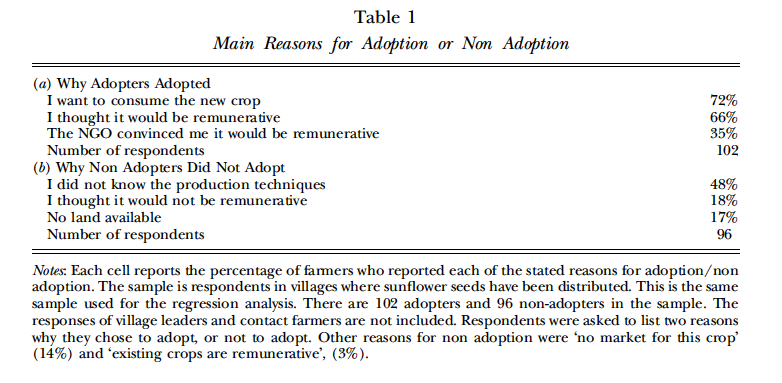
\includegraphics[width=\textwidth]{01table1}
   \label{fig:01table1}
\end{centering}
\end{figure}
\end{frame}

\begin{frame}{Effect of social network on technology adoption}{}
\begin{figure}[h]
\begin{centering}
  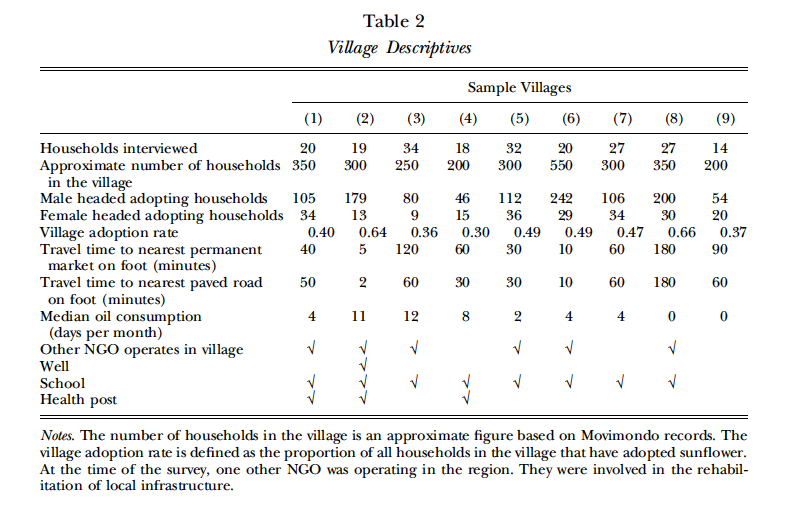
\includegraphics[width=\textwidth]{01table2}
   \label{fig:01table2}
\end{centering}
\end{figure}
\end{frame}

\begin{frame}{Effect of social network on technology adoption}{}
\begin{figure}[h]
\begin{centering}
  \includegraphics[width=\textwidth]{01table3}
   \label{fig:01table3}
\end{centering}
\end{figure}
\end{frame}

\begin{frame}{Effect of social network on technology adoption}{}
\begin{figure}[h]
\begin{centering}
  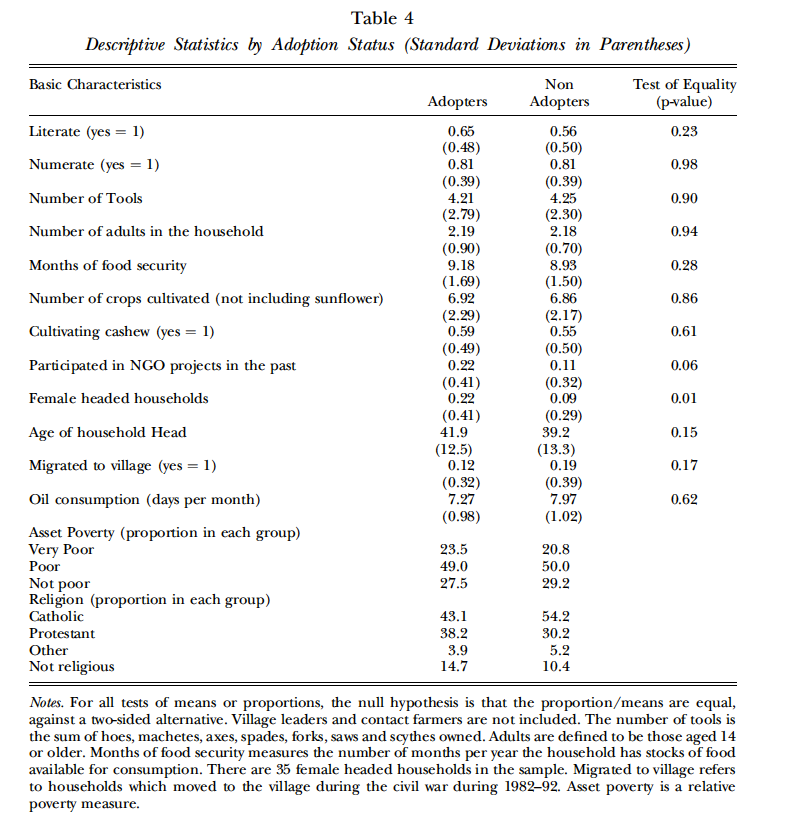
\includegraphics[width=0.7\textwidth]{01table4}
   \label{fig:01table4}
\end{centering}
\end{figure}
\end{frame}

\begin{frame}{Effect of social network on technology adoption}{}
\begin{figure}[h]
\begin{centering}
  \includegraphics[width=\textwidth]{01table5a}
   \label{fig:01table5a}
\end{centering}
\end{figure}
\end{frame}

\begin{frame}{Effect of social network on technology adoption}{}
\begin{figure}[h]
\begin{centering}
  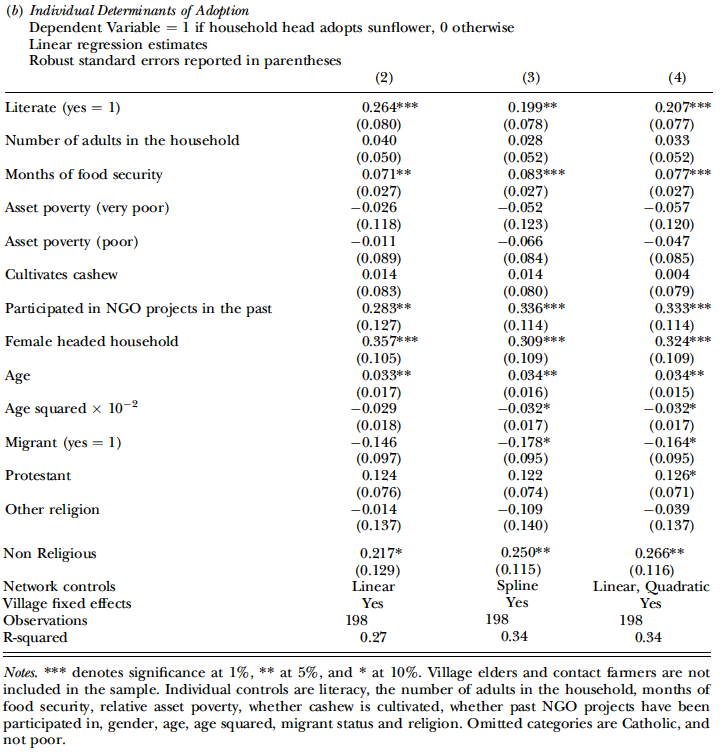
\includegraphics[width=0.6\textwidth]{01table5b}
   \label{fig:01table5b}
\end{centering}
\end{figure}
\end{frame}

\begin{frame}{Effect of social network on technology adoption}{}
\begin{figure}[h]
\begin{centering}
  \includegraphics[width=0.8\textwidth]{01table6}
   \label{fig:01table6}
\end{centering}
\end{figure}
\end{frame}

\begin{frame}{Effect of social network on technology adoption}{}
\begin{figure}[h]
\begin{centering}
  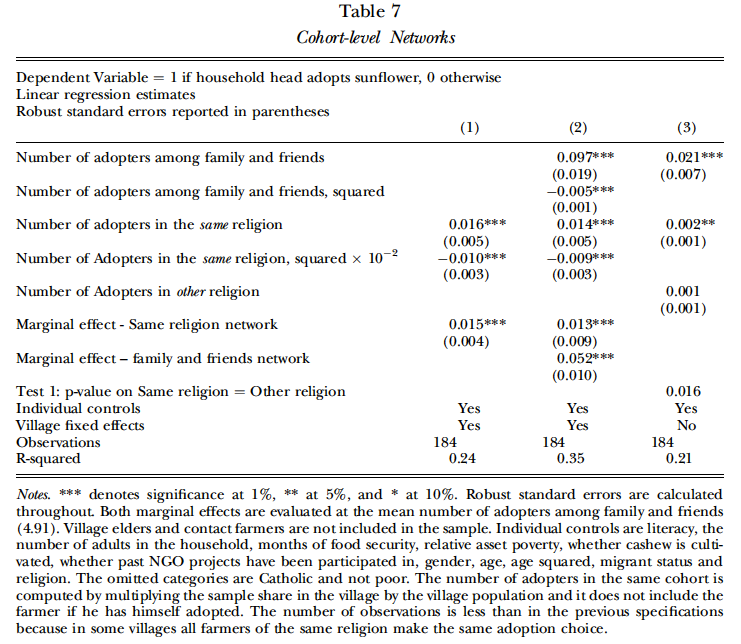
\includegraphics[width=0.8\textwidth]{01table7}
   \label{fig:01table7}
\end{centering}
\end{figure}
\end{frame}

\begin{frame}{Effect of social network on technology adoption}{}
\begin{figure}[h]
\begin{centering}
  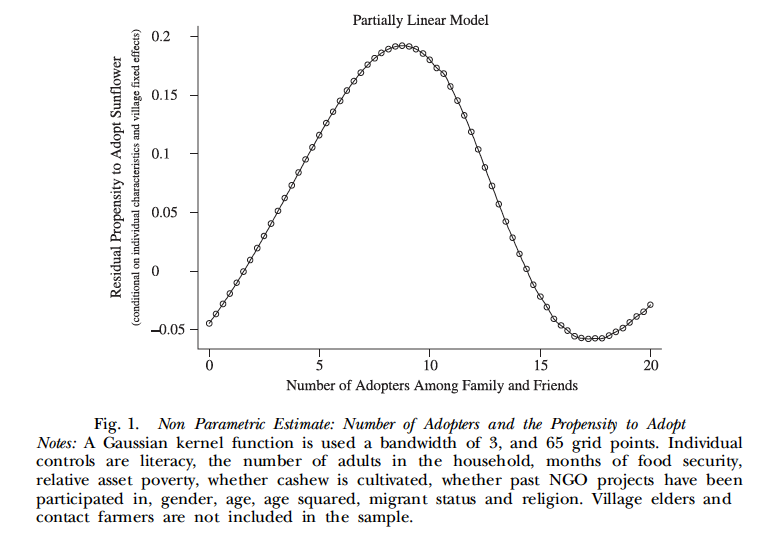
\includegraphics[width=\textwidth]{01fig1}
   \label{fig:01fig1}
\end{centering}
\end{figure}
\end{frame}

\begin{frame}{Effect of social network on technology adoption}{}
\begin{figure}[h]
\begin{centering}
  \includegraphics[width=\textwidth]{01tablea1}
   \label{fig:01tablea1}
\end{centering}
\end{figure}
\end{frame}


\section{\cite{Aghion2005}}
\begin{frame}{Competition and Innovation}{Summary}
\begin{itemize}
\item{Inverted-U relationship between competition and innovation}
\item{Model: Escape-competition effect - increasing profit from innovation}
\item{Model: Schumpeterian effect - reduction in innovation incentives for laggards}
\item{Degree of technological neck-and-neckness should decrease with higher product market competition}
\item{Higher degree of heck-and-neckness should imply a steeper inverted-U relationship}
\end{itemize}
\end{frame}

\begin{frame}{Competition and Innovation}{}
\begin{figure}[h]
\begin{centering}
  \includegraphics[width=\textwidth]{0201}
   \label{fig:0201}
\end{centering}
\end{figure}
\end{frame}


\begin{frame}{Competition and Innovation}{}
\begin{figure}[h]
\begin{centering}
  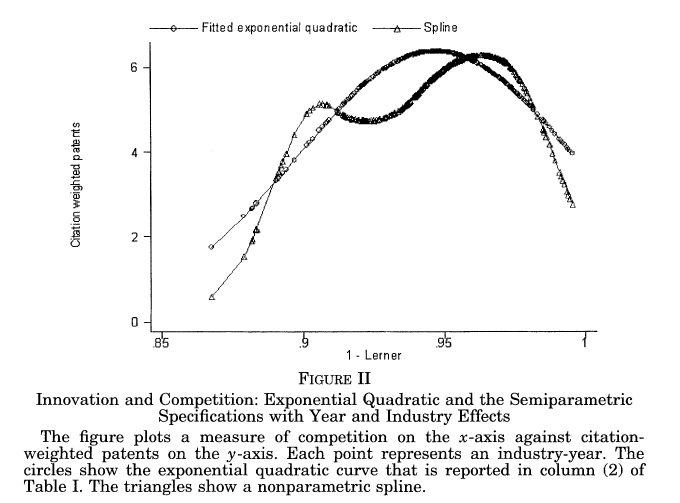
\includegraphics[width=\textwidth]{0202}
   \label{fig:0202}
\end{centering}
\end{figure}
\end{frame}

\begin{frame}{Competition and Innovation}{}
\begin{figure}[h]
\begin{centering}
  \includegraphics[width=0.7\textwidth]{0203}
   \label{fig:0203}
\end{centering}
\end{figure}
\end{frame}

\begin{frame}{Competition and Innovation}{}
\begin{figure}[h]
\begin{centering}
  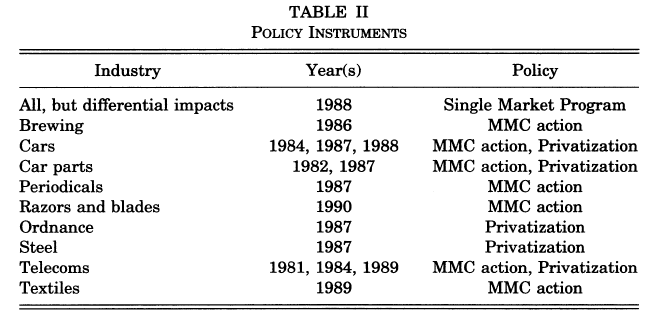
\includegraphics[width=\textwidth]{0204}
   \label{fig:0204}
\end{centering}
\end{figure}
\end{frame}

\begin{frame}{Competition and Innovation}{}
\begin{figure}[h]
\begin{centering}
  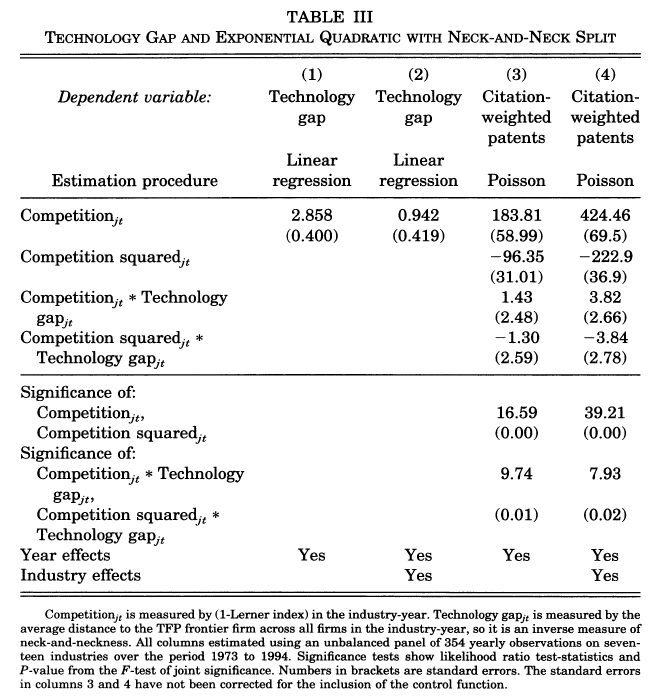
\includegraphics[width=0.7\textwidth]{0205}
   \label{fig:0205}
\end{centering}
\end{figure}
\end{frame}

\begin{frame}{Competition and Innovation}{}
\begin{figure}[h]
\begin{centering}
  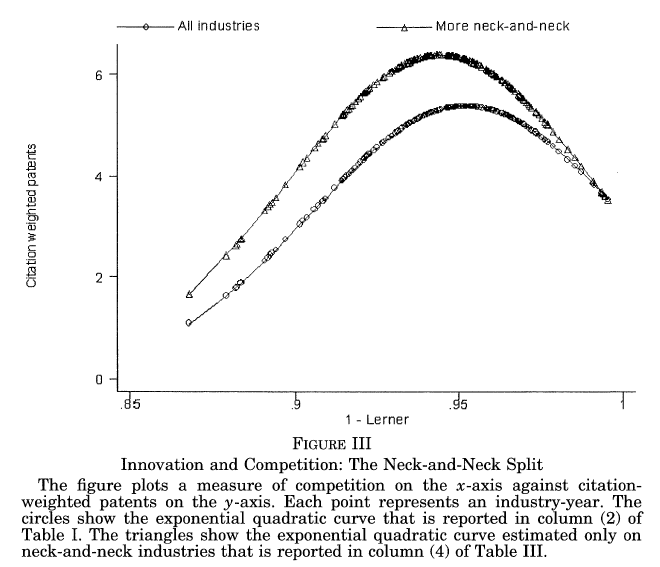
\includegraphics[width=0.8\textwidth]{0206}
   \label{fig:0206}
\end{centering}
\end{figure}
\end{frame}

\begin{frame}{Competition and Innovation}{}
\begin{figure}[h]
\begin{centering}
  \includegraphics[width=\textwidth]{0207}
   \label{fig:0207}
\end{centering}
\end{figure}
\end{frame}


\section{\cite{Arora2001}}
\begin{frame}{Markets for Technology}{Summary}
\begin{itemize}
\item{Technology Users: Markets for Technology allow for licensing in addition to internal exploitation}
\item{Tradeoff: Profit dissipation effect vs. Revenue effect - distant market, lower licensor share, highly competitive downstream market}
\item{Imporved internal management and organization of company intellectual property}
\item{Small firms and Technology startups: Increase effectiveness based on specialization}
\item{Lack of complementary assets does not require them to incur costly and risky downstream investments}
\item{Technology Buyers: Increase in penalty of the not invented here syndrome, reduce relative importance of technology as source of distinct advantage}
\item{Firms may increase in downstream differntiation}
\end{itemize}
\end{frame}

\begin{frame}{Markets for Technology}{}
\begin{figure}[h]
\begin{centering}
  \includegraphics[width=\textwidth]{0301}
   \label{fig:0301}
\end{centering}
\end{figure}
\end{frame}

\begin{frame}{Markets for Technology}{}
\begin{figure}[h]
\begin{centering}
  \includegraphics[width=\textwidth]{0302}
   \label{fig:0302}
\end{centering}
\end{figure}
\end{frame}

\section{\cite{Cohen1990}}
\begin{frame}{Absorptive Capacity}{Summary}
\begin{itemize}
\item{R\&D creates capacity to assimilate and exploit new knowledge}
\item{Firms may conduct basic research less for particular results, but for building absorptive capacity}
\item{Ease of learning affected by degree to which an innovation is related to pre-existing knowledge base}
\item{Explanation for cooperative research ventures}
\end{itemize}
\end{frame}

\begin{frame}{Absorptive Capacity}{}
\begin{figure}[h]
\begin{centering}
  \includegraphics[width=\textwidth]{0401}
   \label{fig:0401}
\end{centering}
\end{figure}
\end{frame}

\begin{frame}{Absorptive Capacity}{}
\begin{figure}[h]
\begin{centering}
  \includegraphics[width=\textwidth]{0402}
   \label{fig:0402}
\end{centering}
\end{figure}
\end{frame}

\begin{frame}{Absorptive Capacity}{}
\begin{figure}[h]
\begin{centering}
  \includegraphics[width=0.55\textwidth]{0403}
   \label{fig:0403}
\end{centering}
\end{figure}
\end{frame}

\bibliography{/Users/aiyenggar/OneDrive/code/bibliography/ae,/Users/aiyenggar/OneDrive/code/bibliography/fj,/Users/aiyenggar/OneDrive/code/bibliography/ko,/Users/aiyenggar/OneDrive/code/bibliography/pt,/Users/aiyenggar/OneDrive/code/bibliography/uz}
\bibliographystyle{apalike}

\end{document}




\begin{comment}
\begin{figure}[h]
\begin{centering}
  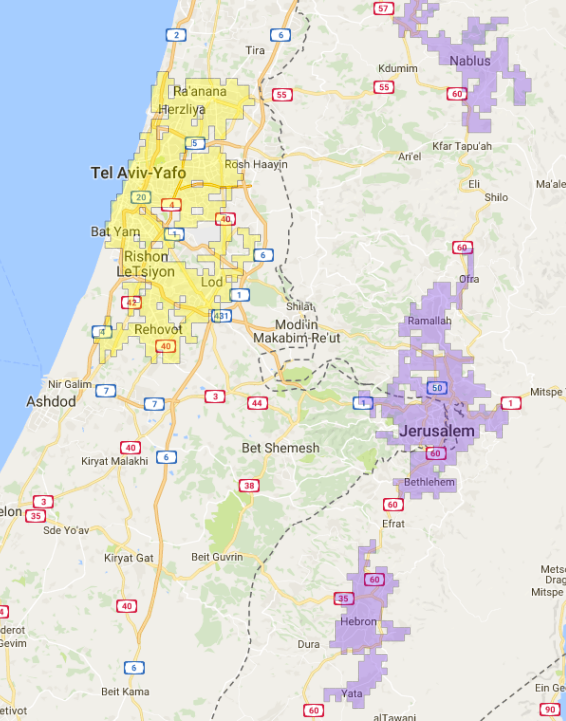
\includegraphics[width=\textwidth]{TelAviv}
  \caption{Geographic Definition of Tel Aviv-Yafo}
   \label{fig:TelAviv}
\end{centering}
\end{figure}
\end{comment}

